%-----------------------------------------------%
% Início do plano de aula
%-----------------------------------------------%
\thispagestyle{empty}
\begin{center}
	\begin{minipage}[!]{\linewidth}
        \begin{minipage}[!]{.19\linewidth}
            
\includegraphics[width=\linewidth]{img/logo.png}           
        \end{minipage}
        \begin{minipage}[!]{.8\linewidth}
            \center
            \ABNTEXchapterfont\normalsize\MakeUppercase{\imprimirinstituicao}
            \par
            \vspace*{10pt}                     
            \ABNTEXchapterfont\normalsize\MakeUppercase{\centro}
            \par
            \vspace*{10pt}           
            \ABNTEXchapterfont\normalsize\MakeUppercase{\disciplina}
        \end{minipage}        
    \end{minipage}
    \\ \vspace{0.5cm}
    \rule{\textwidth}{.5pt}   
\end{center}
    \textual
    \begin{center}
      \section{Ondas I}
      \par
    \end{center}
    
    \noindent \textbf{Estagiário(a): }\imprimirautor 
    
    \noindent \textbf{U.E.:} EEB Giovani Pasqualini Faraco
    
    \noindent \textbf{Série:} 2º Ano\hfill{}\textbf{Turma:} 2º--5
    
    \noindent \textbf{Aula:} 004\hfill{}\textbf{Data:} 21/10/2022\hfill{}\textbf{Duração:} $45\min$
    \rule{\textwidth}{.5pt}
    \bigskip{}  
    

    \noindent
    \begin{center}
      \textbf{Ondas: Grandezas Descritivas}
    \par\end{center}
    \vspace{20pt}
    \par\noindent\textbf{Resumo da aula:} Será introduzido o conceito de ondas de forma a dar suporte ao estudo da propagação luminosa, nesse formalismo.
    \vspace{20pt}
    \par\noindent \textbf{Habilidades BNCC:} EF09CI06; EF09CI04.    
    \vfill     
    \subsection*{Objetivo de Aprendizagem}
    \begin{itemize}
        \item Conhecer as principais grandezas do movimento oscilatório;
        \item Calcular a velocidade de uma onda qualquer com base em suas grandezas constituintes.
    \end{itemize}
    \medskip{}
    \vfill  
    \noindent \textbf{Núcleo Conceitual:} \emph{Ondulatória; comprimento de onda; período e frequência.}

    \newpage
    \section*{Procedimento Didático} 
    \noindent \emph{1º Momento:} Introdução ao modelo ondulatório
    \par\noindent\rule{.3\textwidth}{.5pt}  
    \par\noindent \textbf{Tempo previsto:} 10 minutos

    \noindent \textbf{Dinâmica:} Na aula passada vimos como descrever os fenômenos de reflexão e a refração da luz usando o modelo corpuscular construído por Newton.

    Conduzir a turma para a  síntese obtida na aula passada, em que: o ângulo de incidência e o ângulo refletido são sempre iguais, concordando com o que observa-se para o fenômeno, e para a refração, o modelo corpuscular, prevê uma velocidade maior da luz em meios mais densos como a água, do que em meios menos densos como o ar.

    Citar que a teoria newtoniana não era a única que buscava uma melhor compreensão para os fenômenos luminosos, havia naquela época, uma teoria concorrente baseada em observações que também se propunha a explicar estes fenômenos, mas de maneira diferente, a teoria ondulatória da luz, defendida principalmente por Christiaan Huygens (1629– 1695). 

    Para compreender melhor este modelo, precisaremos conhecer algumas grandezas relacionadas ao movimento oscilatório.

    \vspace*{20pt}
    \noindent \emph{2º Momento:} Grandezas fundamentais do movimento oscilatório
    \par\noindent\rule{.3\textwidth}{.5pt}  
    \par\noindent \textbf{Tempo previsto:} 20 minutos

    \noindent \textbf{Dinâmica:} Esquematizar no quadro o desenho de uma onda propagando-se em uma corda, e definir o comprimento de onda $\lambda$ como a distância entre dois picos ou dois vales consecutivos. O quadro deve ficar mais ou menos similar a \autoref{fig:comprimento-de-onda} a seguir:
    \vspace*{20pt}
    \begin{figure}[!ht]
        \centering
        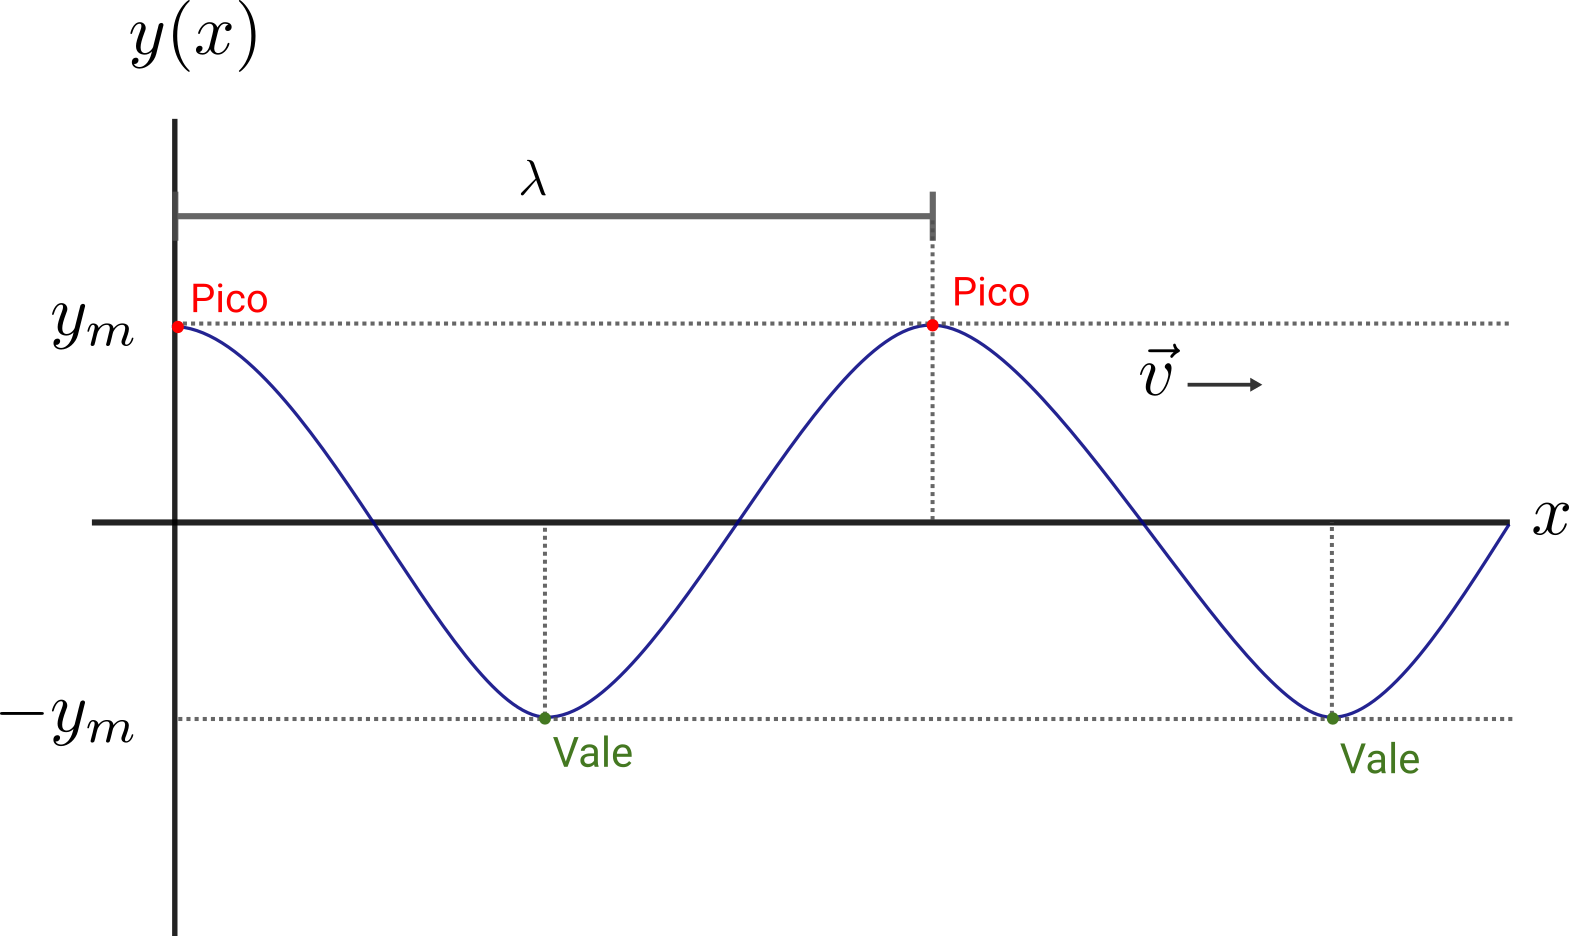
\includegraphics[width=0.6\textwidth]{img/lambda-1.png}
        \caption{Comprimento de onda $\lambda$ em uma corda}
        \label{fig:comprimento-de-onda}
    \end{figure}
    \vspace*{20pt}

    De forma similar, definir o período de uma onda em uma corda, como o intervalo de tempo necessário para que a onda complete um ciclo de oscilação. A medir que for introduzindo os conceitos, desenhar no quadro uma figura semelhante a \autoref{fig:periodo-de-onda} para auxiliar a compreensão dos estudantes.

    \vspace*{20pt}
    \begin{figure}[!ht]
        \centering
        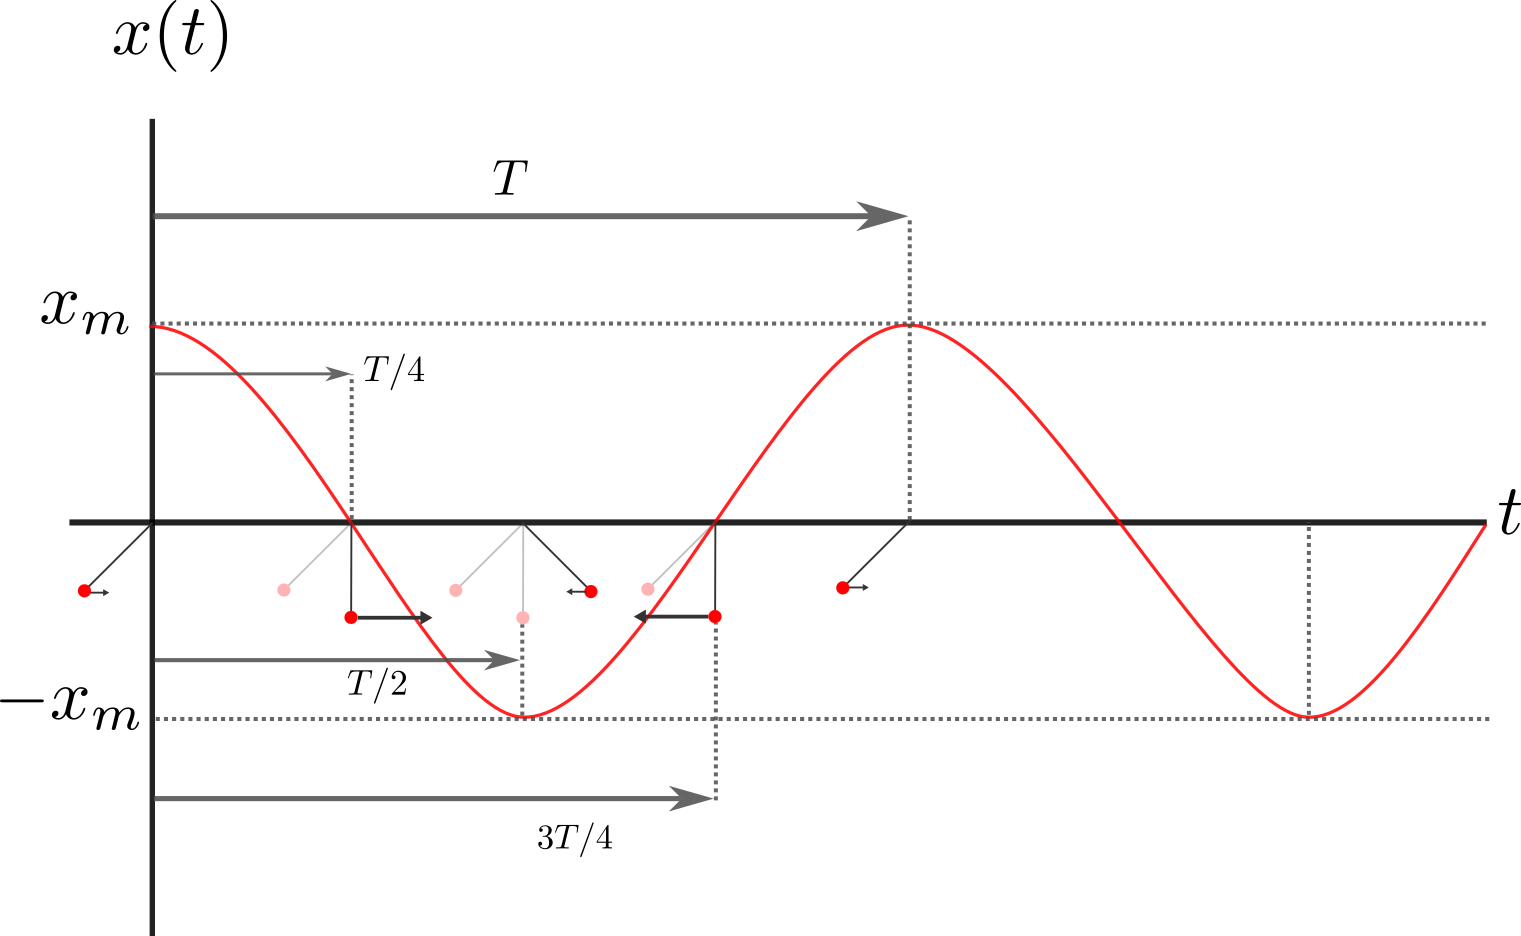
\includegraphics[width=0.6\textwidth]{img/periodo-1.png}
        \caption{Período $T$}
        \label{fig:periodo-de-onda}
    \end{figure}
    \vspace*{20pt}

    Definir a frequência como a quantidade de ciclos que a onda completa em um intervalo de tempo determinado.
    \begin{align}
        f&=\frac{1}{T}
    \end{align}

    \vspace*{20pt}
    \noindent \emph{3º Momento:} Velocidade de uma onda
    \par\noindent\rule{.3\textwidth}{.5pt}  
    \par\noindent \textbf{Tempo previsto:} 15 minutos

    \noindent \textbf{Dinâmica:} A velocidade de propagação de uma onda pode ser calculada usando o conceito de velocidade escalar média visto no primeiro ano.

    \begin{align}
        v&=\frac{\Delta S}{\Delta t}
    \end{align}

    Esta relação para uma onda fica

    \begin{align}
        v&=\frac{\lambda}{T}
    \end{align}
    o que também pode ser escrito em termos da frequência como
    \begin{align}
        v&=\lambda f
    \end{align}

    Após estabelecida a equação da velocidade de uma onda, pedir que diferentes grupos de alunos estimem a velocidade das ondas do espectro visível a partir dos dados da \autoref{tab:alguns-espectros-do-visivel}:
    \vspace*{1pt}
    
    \begin{table}[!ht]
        \centering
        \begin{tabular}{|c|c|c|}
        \hline
        \textbf{Cor}      & \textbf{$\lambda(\textrm{nm})$} & \textbf{Frequência $f(10^{12}\textrm{Hz})$} \\ \hline
        \textbf{Vermelho} & 625                             & 480                                         \\ \hline
        \textbf{Laranja}  & 590                             & 510                                         \\ \hline
        \textbf{Amarelo}  & 565                             & 530                                         \\ \hline
        \textbf{Verde}    & 500                             & 600                                         \\ \hline
        \end{tabular}
        \caption{Comprimentos de onda $\lambda$ e frequências $f$ de algumas faixas de valores do espectro visível.}
        \label{tab:alguns-espectros-do-visivel}
    \end{table}
    \vspace*{10pt}

    \noindent Todos devem encontrar valores muito próximos a $2,99\times 10^8\mps$. Questionar o motivo pelo qual todos encontraram valores muito próximos, e se já conhecem este valor de velocidade. Relacionar esta velocidade com a velocidade da luz no vácuo e justificar que pelo fato do ar, ser o meio material cujo o qual oferece a menor resistência à passagem da luz, os físicos normalmente utilizam a velocidade da luz no ar igual à velocidade da luz no vácuo.
    
    Análogo ao que foi feito pra velocidade da luz, sugerir que a partir da \autoref{tab:notas-musicais} logo a abaixo estimem a velocidade do som
    \vspace*{10pt}
    
    \begin{table}[!ht]
        \centering
        \begin{tabular}{|c|c|c|}
        \hline
        \textbf{Nota} & \textbf{$\lambda(\textrm{m})$} & \textbf{Frequência $f(\textrm{Hz})$} \\ \hline
        \textbf{C}    & 21,04                          & 16,35                                \\ \hline
        \textbf{D}    & 18,74                          & 18,35                                \\ \hline
        \textbf{E}    & 16,70                          & 20,60                                \\ \hline
        \textbf{F}    & 15,76                          & 21,82                                \\ \hline
        \textbf{G}    & 14,04                          & 24,50                                \\ \hline
        \textbf{A}    & 12,51                          & 27,50                                \\ \hline
        \textbf{B}    & 11,14                          & 30,86                                \\ \hline
        \end{tabular}
        \caption{Comprimentos de onda $lambda$ e frequências $f$ de algumas notas musicais.}
        \label{tab:notas-musicais}
    \end{table}
    \vspace*{10pt}
    
    Dedicar o restante da aula para discussão destes resultados e tiragem de dúvidas sobre a exposição.

    